

\newcommand{\amel}[1]{{\color{orange} #1}} 

\section*{Reproducibility Summary}


\subsubsection{Scope of Reproducibility}

In this work, the article Predicting Dynamic Embedding Trajectory in Temporal Interaction Networks~\cite{kumar2019predicting} is evaluated through a replication study. Replication results examine whether the claims made by authors are valid. Our goal is to replicate the experiments and achieve the same results as the authors.

\subsubsection{Methodology}

We reimplement the method of Kumar et al.~\cite{kumar2019predicting} for recommender systems using their new algorithm that allows batch learning on temporal data, improves their codes, and extends their work. Our improvements consist of using the last versions of Python and  Pytorch, and having a more readable code. Our extension includes impacting hyperparameters by varying it. The codes are available at \href{https://github.com/ComplexNetTSP/JODIE}{GitHub}. 

\subsubsection{Result}

We mainly reach the same results with our own code compared to the original paper, with a notable difference with the prediction of future interaction task (with the LastFM dataset) where we achieve a result twice better than the one publish in the paper. Moreover, we showed that the number of split during the learning phase (the number of times the back propagation is performed) has a strong impact on the final results (cf. Fig. \ref{split}). This fact was not highlighted in the original paper.

\subsubsection{What was easy}

The authors had made their code available and all the necessary information at the following  address \href{https://github.com/srijankr/jodie}{GitHub}. Their original code has considerably simplified our replication task.

\subsubsection{What was difficult}

Although the code is available. However some technical aspects have hindered our complete understanding of the model. We solved them by studying the code made available by the authors.

\subsubsection{Communication with original authors}
We contacted the authors for clarification about which aggregation method used to fit the inputs constraints of the RNN gate.

\newpage

\section*{Introduction}

Recommender systems are systems that cover a broad scope of techniques which all aim to provide suggestions of items that are most pertinent to a particular user (e.g., which music playlists to choose, which book a user might like, etc.), see~\cite{Ricci_Rokach_Shapira_2021} for a review of the techniques and challenges of the field. We can observe, particularly in areas such as  e-commerce or social media, that one user may interact with several items/products, and these interactions may evolve with time and context (e.g., Winter clothes recommendations should be different from summer clothes recommendation). 
As a result,  understanding and modeling the dynamic evolution of users and items is an important issue. In the literature, this dynamicity is generally modeled by an embedding trajectory in a Euclidean space. However, existing works suffer from several limitations, as the authors in \cite{kumar2019predicting} pointed out. At first, none of the existing methods predicts the future embedding trajectory. Instead, embeddings are generated only at each user's action. Moreover, static and dynamic properties are generally not considered in the same framework. Finally, scalability remains an open issue for the prediction of user-item interactions as well as for the model's training when dealing with large-scale datasets. To overcome these limitations, \cite{kumar2019predicting} proposes JODIE, a deep learning-based recommender system that models user‐item interactions as a sequence of timestamped edges on a bipartite graph (cf. fig.~\ref{bipartite_graph}).
The core idea is that each user and item has two embeddings: a static embedding representing the entity's long‐term stationary property
and a dynamic embedding representing the time‐varying property. These embeddings are used to make predictions regarding future interactions. The proposed method is trained with batches of data to overcome the scalability issue.
The authors claim to outperform some of the state-of-the-art recommender systems such as Time-LSTM~\cite{Zhu17}, LatentCross~\cite{Beutel18}, Interaction Graph Embedding (IGE)~\cite{Zhang17}, Recurrent Recommender Networks~\cite{Wu17} and the Continuous-Time Dynamic Network Embeddings(CTDNE)~\cite{Nguyen18} in predicting future interactions  at least 20\% better, and user state change predictions 12\% better on average.
This paper describes our efforts to replicate the JODIE model designed by Srijan Kumar et al~\cite{kumar2019predicting}. 
We use the publicly available code provided by the authors to reproduce
their results and validate their conclusions. Our code is available at \href{https://github.com/ComplexNetTSP/JODIE}{Github}.


%%%%%%%%%%%%%%%%%%%%%%%%%%%%%%%%%%%%%%%%%%%%%%%%%%%%%%%%%%%%%%%%%%%%%%%%%%%%%%%%%%%%%%%%%%%%%%%%%%%%%%%%%%%%%
%
% Fig 1
%
%%%%%%%%%%%%%%%%%%%%%%%%%%%%%%%%%%%%%%%%%%%%%%%%%%%%%%%%%%%%%%%%%%%%%%%%%%%%%%%%%%%%%%%%%%%%%%%%%%%%%%%%%%%%%
\begin{figure}[htbp]
    \centering
    \includegraphics[width = 0.2\textwidth]{image/bipartite_graph.pdf}
    \caption{Bipartite graph}
    \label{bipartite_graph}
\end{figure}


\section*{Scope of Reproducibility}

In this paper, we investigate the following claims from the original paper:
\begin{itemize}
    \item \textbf{More accurate recommendation performance}. By using the JODIE model, the authors claim xto achieve better predictions of future interactions over all the selected datasets. JODIE outperforms six models with an improvement of at least 20\% \href{https://github.com/ComplexNetTSP/JODIE}{Github}.  and 14\%  in terms of Mean Reciprocal Rank (MRR) and Recall@10, respectively.
    \item \textbf{More accurate state changes performance}. The authors claim that JODIE outperforms five models regarding the user state change over all the selected datasets with an average improvement of 12.63\% for the Area Under the Curve (AUC) metric.
    \item \textbf{Shorter learning time}. Thanks to the new t-batch algorithm, the learning phase is 9.2 times faster than other models comparable to JODIE, i.e., with a model with two Recurrent Neural Networks (RNNs).
    \item \textbf{Robustness of the model to the proportion of the training set}. Regardless of the training data percentage, JODIE outperforms all the compared models.
    \item \textbf{Robustness of the model to the embedding size}. The size of embeddings does not have much impact on the performance of JODIE.
\end{itemize}
We have implemented the JODIE model using a more recent version of the Pytorch library aiming at reproducing the results stated by the authors:
\begin{itemize}
    \item We explored which embedding size is the most effective for predicting state change and future interaction.
    \item We also replicated the experiments that concern the robustness of the JODIE model to the percentage of training data.
    \item To measure the robustness to dynamic embedding size, the authors measured the performance of JODIE with embedding sizes from 32 to 256 on solely the LastFM dataset. We extended this experiment by adding three embedding sizes, 8, 16, and 32, on the LastFM and Wikipedia datasets and calculating the MRR and Recall@10.
\end{itemize}
In addition to reproducing the results presented in the paper, we perform novel experiment that test the impact of the hyperparameter \texttt{split}. We varied \texttt{split} by 5, 500 and 50000 on the MOOC dataset, which will increase the number of back propagation, and we calculate the performance in AUC. The main issue we encountered during our code replication of the original model~\cite{kumar2019predicting} was the lack of understanding of the \texttt{t-batch} algorithm which is not provided in the original paper and not referenced, but previously publish by the same authors as a \textit{preprint} in \cite{kumar18}.
To conclude, we have reproduced the results present in the original paper by extending an experiment on the robustness of the size of dynamic embeddings and by bringing an additional experiment on the choice of hyperparameters.

\section*{Methodology}
JODIE is a model that learns dynamic embeddings of users $u_t \in \mathbb{R}^n$, $\forall u \in \mathcal{U}$ and items $i_t \in \mathbb{R}^n$, $\forall i \in \mathcal{I}$ over time t, $\forall t \in [0; T]$, where $\mathcal{U}$ and $\mathcal{I}$ are the sets of users and items and $T$ the final time. Moreover, the interactions are ordered in time, i.e., an interaction between a user $u_r$ and an item $i_r$ at time $t_r$ characterized by $f_r$, noted $S_r = (u_r, \, i_r, \, t_r, \, f_r)$, cannot be before the interaction $S_{r-1}$. Figure \ref{Pipeline} shows the structure of JODIE. The model is composed of two main components: the update operator which, with the help of two RNNs, updates embeddings and the projection operator which allows to make a projection of an embedding in a future time represented in purple on the figure. Then, the model uses the different outputs to make the prediction of the future interaction or change of state.


\begin{figure}[H]
    \begin{center}
        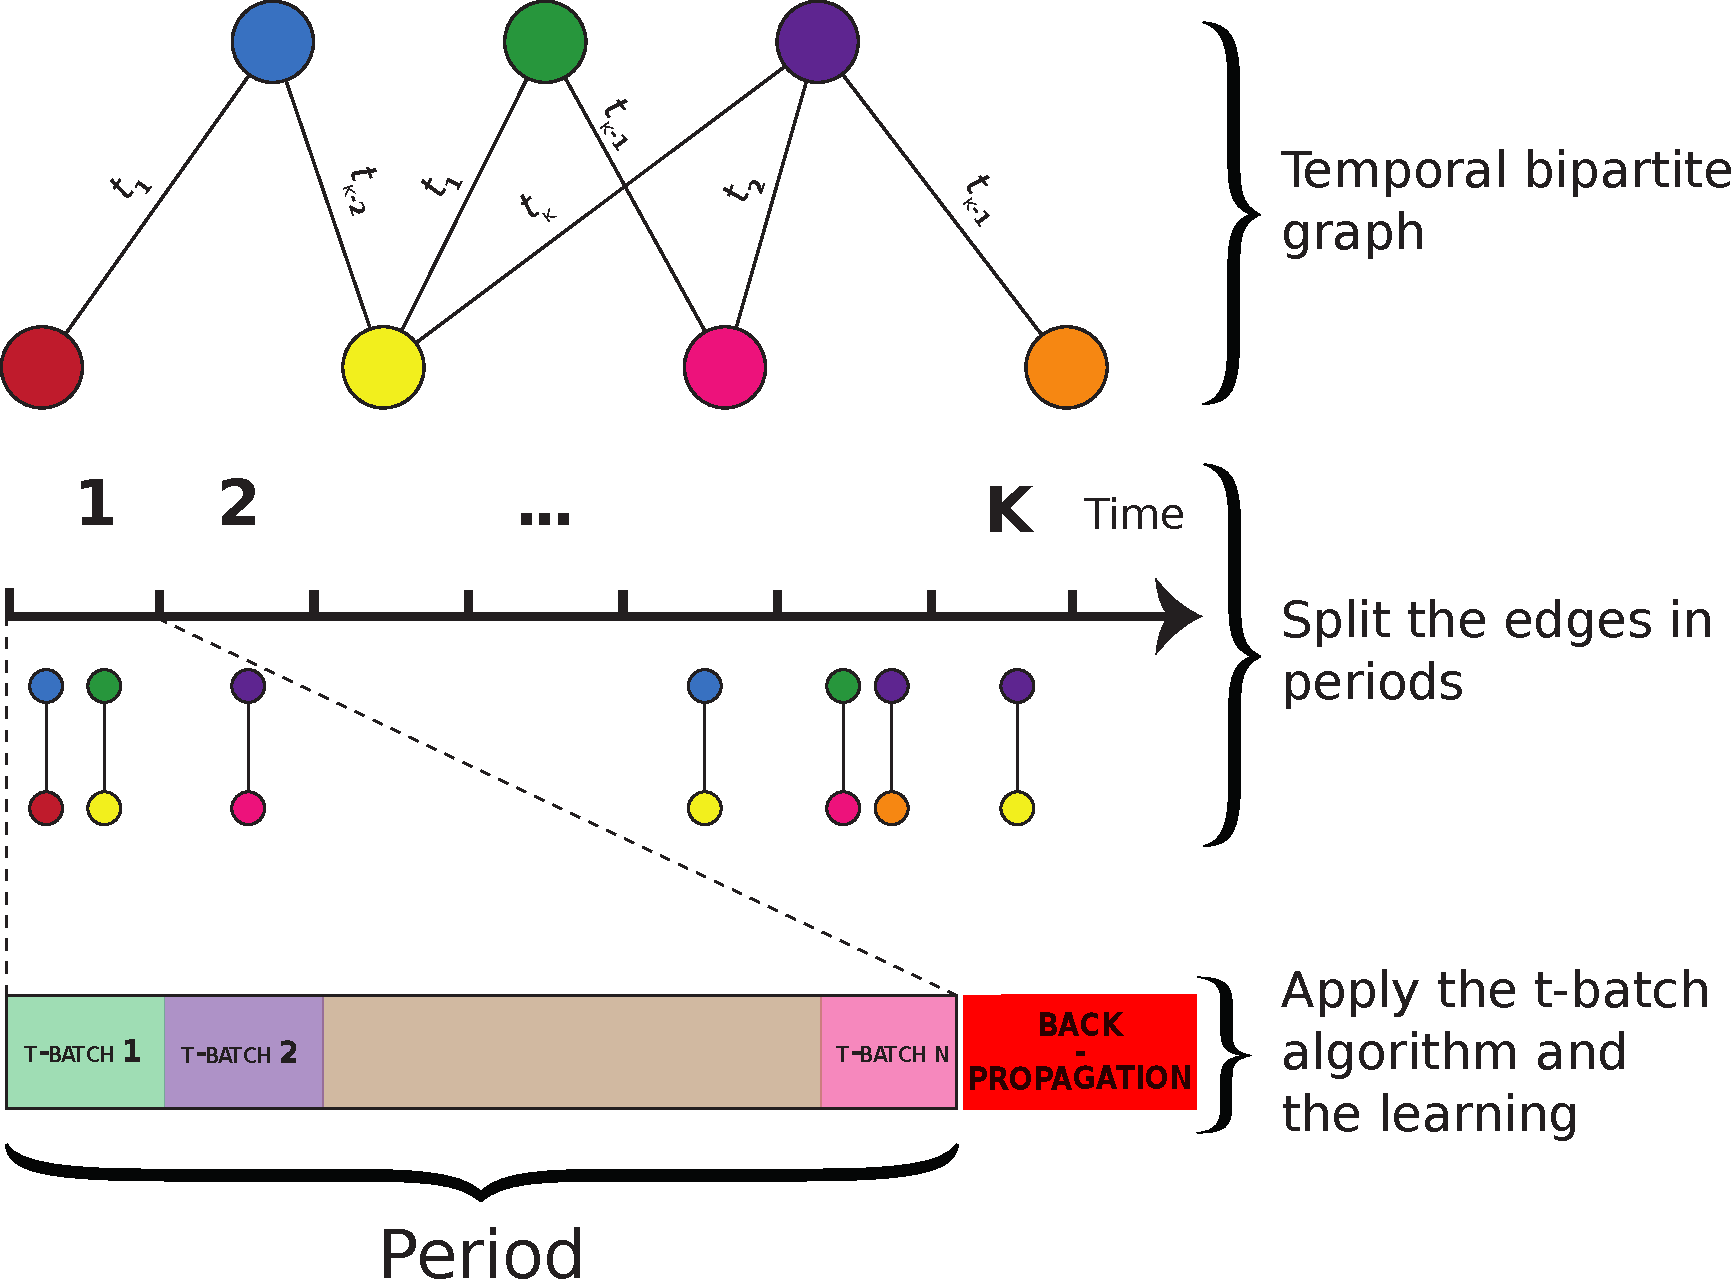
\includegraphics[width=1.0\textwidth]{image/pipeline.pdf}
    \end{center}
    \caption{Pipeline. $MLP_{reg}$ gives an estimation of the embedding of the next item $\textcolor{blue}{\overset{\sim}{i}}$ with which a user $\textcolor{red}{u}$ is likely to interact. The MLP  is designed to recommend the best $\textcolor{blue}{i}$ to each user. $MLP_{classif}$ is used to predict the user's state change $\textcolor{red}{\widehat u_{state}}$. Will the user potentially drop out / get banned ?}
    \label{Pipeline}
\end{figure}

%To better understand what we have done, it is important to see our more recent version of the code, but also the architecture of the model, the loss functions used and the evaluation of JODIE.

\subsection*{Code}
We re-implemented the JODIE model using newer version of Pytorch~\cite{NEURIPS2019_bdbca288} version 1.10 and python 3.8 independently of the original code provided by the authors\footnote{\url{https://github.com/srijankr/jodie}}. We want to highlight the fact that we used the \textit{tanh} function  as the activation function at the output of the RNNs (see fig. \ref{Pipeline}) to build our model,  in accordance to the authors' original code but contrary to what's written in the original paper. Our code is available at the following address: \url{https://github.com/ComplexNetTSP/JODIE}. 

Our source code is organized as follows:
\begin{itemize}
    \item \textbf{preprocessing.py} where everything about the data preprocessing and the t-batch algorithm.
    \item \textbf{model.py} the model as described in figure \ref{Pipeline}.
    \item \textbf{train.py} is used to train the model.
    \item \textbf{evaluate.py} is used to evaluate the model after training.
\end{itemize}
By organizing the work in this way, it allows to have a modular, easily reusable and understandable code.
\textcolor{red}{HOW TO run the Model ....... !!!!!!!!!!!}
\subsection*{Model descriptions}

\subsubsection{Update operator}
% enlever les we
% forme active

The update operator takes the form of two mutually recursive neural networks shown in Figure \ref{recursive RNNs}. The RNN$_U$ is used to update the dynamic user embeddings and the RNN$_I$ updates the dynamic item embeddings. In this case, the embeddings are considered as the hidden state of the classical RNNs respectively. At time $t=0$, the embeddings are initialized randomly according to uniform distribution $\mathcal{U}[0;1[$ followed by a normalization and are noted $u_0$ and $i_0$. As input, there is the embeddings at time $t=0$ but also $\Delta$ the time elapsed between an entity and the previous interaction and $f$ a feature vector which characterizes the link of the interaction. A specificity of these RNNs is that they take four inputs instead of two as usual. In order to narrow down to just two inputs, we concatenate the embedding of the other entity, $\Delta$ and $f$. In Figure \ref{recursive RNNs}, we denote the concatenation by [.,.]. More formally, we use the following formulas to update the embeddings:
$$
u^+ = \sigma \left ( W_1^u u^- + W_2^u i^- + W_3^u f + W_4^u \Delta_u \right )
$$
$$
i^+ = \sigma \left ( W_1^i i^- + W_2^i u^- + W_3^i f + W_4^i \Delta_i \right )
$$
Where the matrices $W_1^e, ..., W_4^e$ are the parameters of the RNN$_e$ and $\sigma$ an activation function (here hyperbolic tangent). We note by $u^-$ and $i^-$ the embeddings before update and by $u^+$ and $i^+$ the embeddings after update. Once this step is finished, we can proceed to the second operation, the projection operation.

\begin{figure}[H]
   \centering
    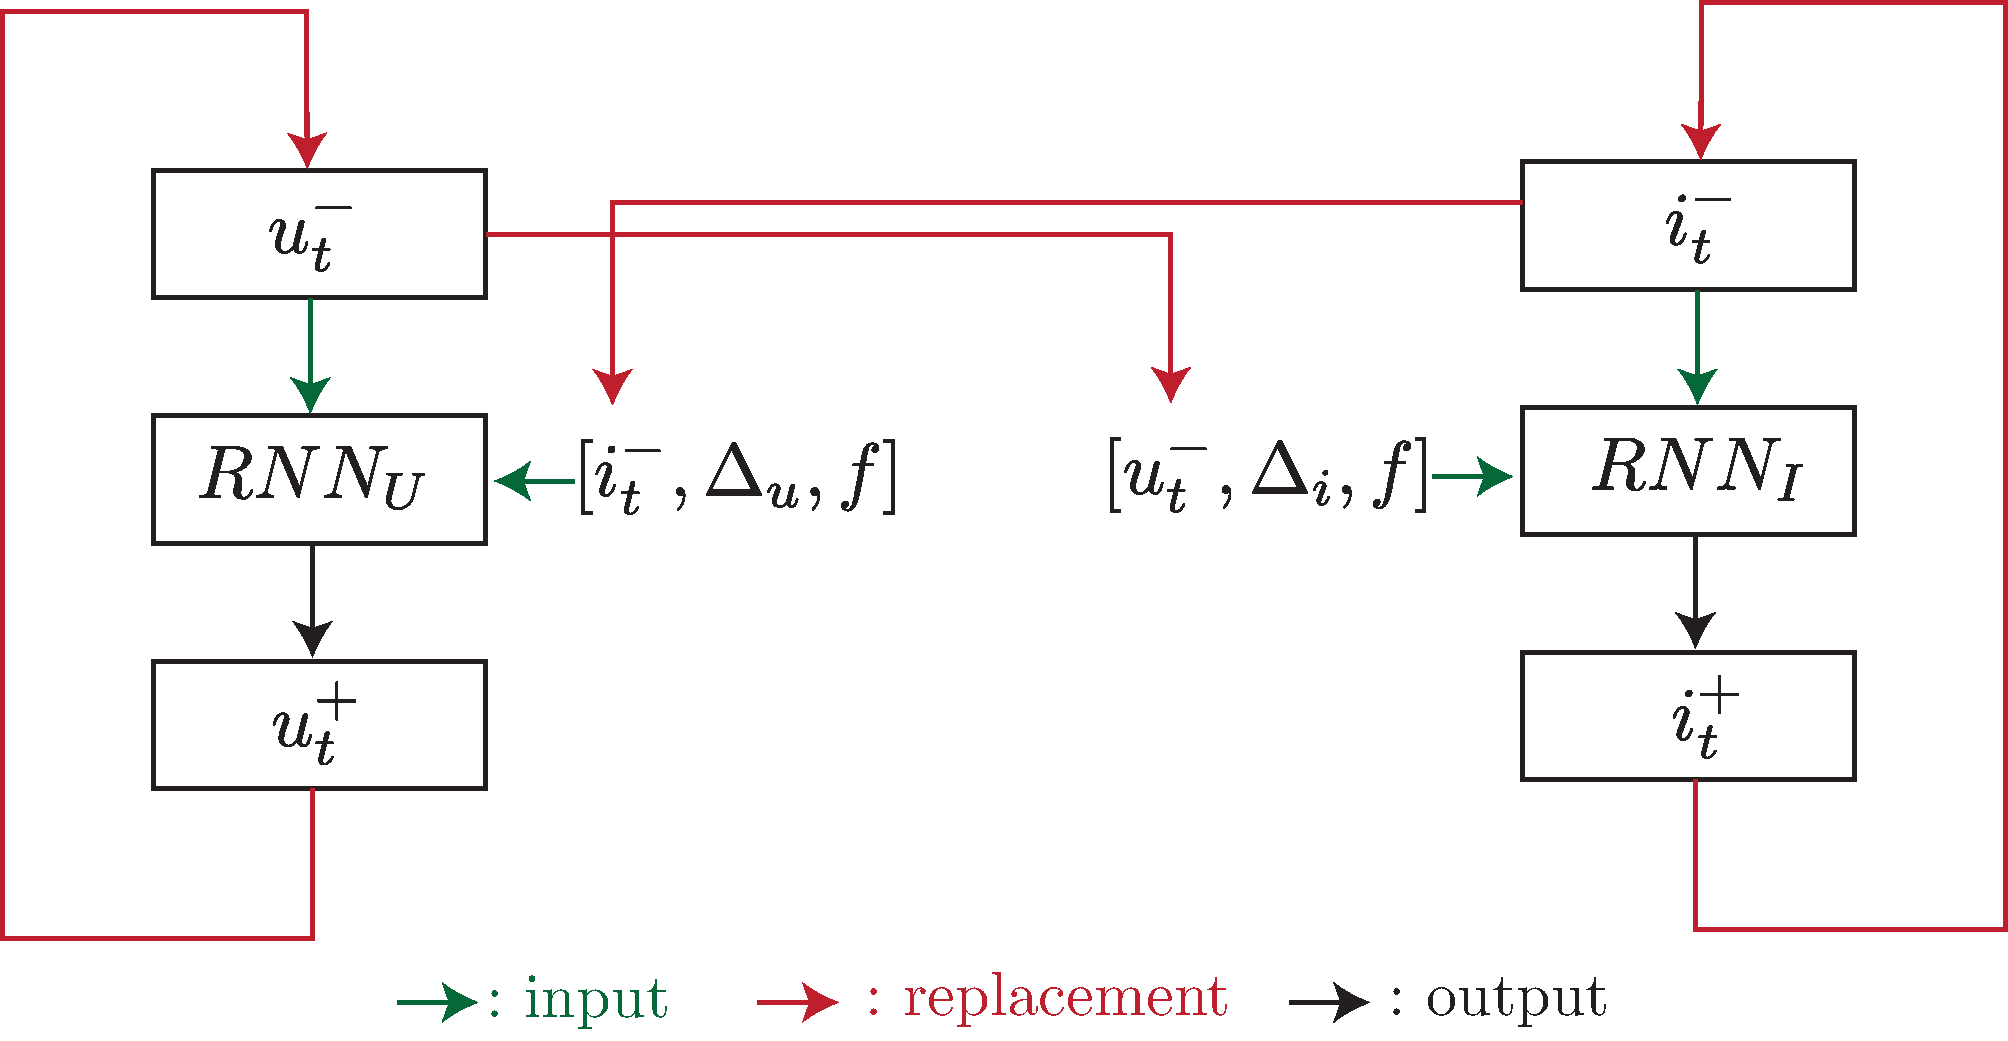
\includegraphics[width=1.0\textwidth]{image/rnn_jodie.pdf}
    \caption{RNN mutually recursive}
    \label{recursive RNNs}
\end{figure}

\subsubsection{Projection operation}

This operation consists in projecting the user's embedding to a future time. Indeed, it is assumed that user's interest changes with time, for example in winter and in summer, hence the need to model this variation as a linear projection. To a more deeper understanding please refer to the orginal figure provide by the authors themself in figure 3 in~\cite{kumar2019predicting}).

We notice that over a very short time interval, the projected embedding of the user changes slightly, but as time goes, the projected embedding will be further away from its original embedding. To perform this operation, we must first convert $\Delta$ into a vector $w \in \mathbb{R}^n$ using a linear layer represented by its weights vector $W_p$. We have $w = W_p \Delta$. We initialize $W_p$ by a Gaussian of zero mean. We obtain the projected embedding by computing Hadamard product, denoted $*$, of $1+w$ and $u_t$. The authors use the following formula.
$$
\widehat u_{t+\Delta} = (1+w) * u_t
$$
We can see that if $\Delta = 0$ then $w=0$ and the projected embedding is the same as the initial embedding. We can consider this operation as a simple linear transformation.

These two operators consist in the learning of the model. One limitation cited by the authors is the learning time. Indeed, the existing models process each interaction one after the other, which takes a considerable amount of time. The authors have invented an algorithm that allows to separate temporal data in batches and thus to accelerate the learning time. This algorithm is called \texttt{t-batch}.

\subsubsection{t-Batch algorithm}

The \texttt{t-batch} algorithm is a linear algorithm that split temporal data into batches. This algorithm is a key point of the method that allows to speed up the learning time considerably. The \texttt{t-batch} algorithm is explained in the original article only by a few lines. Regarding the code, the algorithm was difficult to identify since it was mixed with other parts of code in the learning loop. To facilitate the understanding of the \texttt{t-batch} we propose the following algorithm \ref{t-batch}. To summarize the \ref{t-batch} algorithm, given a list of timestamped events, it dispatches the event into a batch according to the following constrains first it ensures that the same batch cannot contain the same entity multiple times. Secondly, it ensures to retain temporal dependencies inside batches and between batches, i.e., we process interactions in order. By meeting these two conditions, we guarantee that batches are independent (and parallelizable). Finally, in line 9. of Alg. \ref{t-batch} we compute the index of the batch $B_{idx}$ where the interaction $\mathcal{S}_r \in \mathcal{S}$ will be put in. Let $\text{maxBatch}(e, \,r-1)$ be the function that gives the index of the batch at time $r-1$ containing the entity $e$. 

    \begin{algorithm}[H]
        \caption{t-Batch}
        \label{t-batch}
        \begin{algorithmic}[1]
            \STATE \textbf{Input} : Sequence of interactions ordered by time $S$ : $S_j = (u_j,\,i_j,\,t_j,\,f_j)$
            \STATE \textbf{Output} : Sequence of batches $B$ : $B_k = \{S_{k,1},\,...,\,S_{k,n} \}$
            \STATE \textbf{Initialize} : 
            \STATE \quad $\text{tbatch\_id\_u[u]} \leftarrow 0 \; \forall \; u \in \mathcal{U}$, \quad $\text{tbatch\_id\_i[i]} \leftarrow 0 \; \forall \; i \in \mathcal{I}$
            \STATE \quad $B_k \leftarrow \{ \},\; \forall \; k \in$ [\![$1,\;\text{Card}(S)$]\!]
            \STATE \quad $C \leftarrow 0$
            \FOR{$S_j \in S$}
                \STATE Extraction $S_j = (u_j,\,i_j,\,t_j,\,f_j)$
                \STATE idx $\leftarrow$ $\max$(tbatch\_id\_u[$u_j$], tbatch\_id\_i[$i_j$]) + 1
                \STATE $B_\text{idx} \leftarrow B_\text{idx} \cup \{ S_j \}$
                \STATE tbatch\_id\_u[$u_j$] = idx
                \STATE tbatch\_id\_i[$i_j$] = idx
                \STATE $C \leftarrow \max(C,\,$idx)
            \ENDFOR
            \RETURN $\{ B_1,\,...,\,B_C \}$
        \end{algorithmic}
    \end{algorithm}


% \begin{equation}
% \text{idx} = \max \left ( \text{maxBatch}(u, \,r-1), \,\text{maxBatch}(i, \,r-1) \right ) + 1
% \label{eq:1}
% \end{equation}

\subsubsection{Next item embedding and state change losses}

The JODIE model has been designed to give directly an embedding of an item, which is time saving. Indeed, the existing models predict a probability for each item. This can be very long if the dataset contains many items. JODIE will produce an embedding and the suggested item will be the one whose embedding will be the closest to the one of the prediction. To make this prediction, we use a neural network that will have as input the projected embedding of the user at time $t+\Delta$ noted $\widehat u(t+\Delta)$ and the embedding of the previous item of the user before time $t+\Delta$ noted $i(t+\Delta^-)$. This embedding is important because item can interact with other users between time $t$ and $t+\Delta$, which means that it contains more recent information. JODIE uses both static and dynamic embeddings, denoted respectively $\Bar{e}$ and $e$, to make the prediction of a static and dynamic embedding $\overset{\sim}{i}$. The prediction is done with a fully connected linear layer.
$$
\overset{\sim}{i} (t+\Delta) = W_1 \widehat u(t+\Delta) + W_2 \Bar{u} + W_3 i(t+\Delta^-) + W_4 \Bar{i} + B
$$
Where $W_1, ..., W_4$ and the bias vector $B$ are the model weights.\\

JODIE is trained to minimize the L2 distance between the predicted embedding and the real item embedding of each interaction. We compute the loss function as follows:

\begin{equation}
    \textit{Loss} = \sum_{(u,\,i,\,t,\,f) \in S} \| \overset{\sim}{i}_t - [\Bar{i},\,i_t^-] \|_2 + \lambda_U \|u_t - u_t^-\|_2 + \lambda_I \|i_t - i_t^-\|_2
\end{equation}

The first term minimizes the error of the predicted embedding. The next twos terms regulate the loss function and allow the dynamic embeddings of users and items to not vary too much. $\lambda_U$ and $\lambda_I$ are the regularization terms that penalize the two terms. In the original paper, the authors fixed the values of $\lambda_U$ and $\lambda_I$ as: $\lambda_U = \lambda_I = 1$, without much justification. It is not clear if this is the best value or if another value would be more appropriate. \\

When we want to predict the change of state of a user, we use the same loss function with an additional term which is the cross-entropy. To do this, we have to make sure that the classes are binary. In this case, it is possible to train the model using an additional loss term function that will make it able to predict the labels using the user's embedding after an interaction. The additional loss function term, for predicting a user's state change, is a weighted cross-entropy expressed in the following equation:

\begin{equation}
    \ell(x,y) = \sum_{n=1}^N \frac{l_n}{\sum_{n=1}^N w_{y_n}} \; \text{ with } \;
    l_n = -w_{y_n} \log \left ( \frac{\exp(x_{n,y_n})}{\sum_{c=1}^C \exp(x_{n,c})} \right )
\end{equation}
rite the corresponding paper using the proposed LaTeX template or your own t
Where $x$ is the input, $y$ is the target, $w$ is the weight, $C$ is the number of classes (here two) and $N$ is the batch size. The loss function becomes:

\begin{equation}
    \textit{Loss} = \sum_{(u,\,i,\,t,\,f) \in S} \| \overset{\sim}{i}_t - [\Bar{i},\,i_t^-] \|_2 + \lambda_U \|u_t - u_t^-\|_2 + \lambda_I \|i_t - i_t^-\|_2 + \ell (u_{true}, \widehat u_{pred})
\end{equation}

Where $u_{true}$ is the real class of the user and $\widehat u_{pred}$ his predicted class. It is also worth noting that the regularizations terms are MSE. The authors wanted the embeddings not to vary heavily between the previous time $t-1$ and the current time $t$. Indeed, they started from the postulate that the behavior of a user represented by its dynamic embedding does not vary considerably over a small temporal interval.\\

\subsubsection{Training JODIE model} 

% bien définir une période et le split dans l'étape 3 pour rendre les choses bien clair et facilité la compréhension.

We detail the learning steps and the specificity of JODIE model we provide. 
\begin{enumerate}
    \item We use a function called \textbf{preprocess} which is in the file \textbf{preprocessing.py} to make a pre-processing of the data to extract information necessary during the training. Information like the sequence of users, items, time, features or previous items that will be used during the learning step.
    \item We initialize each embedding randomly $\mathcal{U}([0,1[)$.
    \item During the trainning phase we usually we split the observations from the original dataset within a given number of batches. But when we have a dataset has a temporal dependency, we cannot operate under the same assumption, that why in the JODIE model they created the \texttt{t-batch} algorithm. First, we split evenly the dataset into ordered batch of data secondly, we apply the \texttt{t-batch} algorithm independently on each subset of the data as described in the figure \ref{pipeline_t-batch}. Our implementation of the \texttt{t-batch} differ from what was originaly defined in \cite{kumar18}, in our implementation do all the t-batches at once with the function \textbf{t\_batch} in the file \textbf{preprocessing.py} before the learning step and loop over the periods.
    \item During the learning stage, in the function \textbf{train\_ray} in the file \textbf{train.py}, we use the function \textbf{projection} from the file \textbf{model.py} to project users' embedding in a future time. We also use the function \textbf{predict\_embedding\_item} in the file \textbf{model.py} to make a prediction of the next embedding of the item. And finally, we calculate the Mean Square Error (MSE) of the predicted embedding and the real embedding.
    \item We update embeddings of users and items using the functions \textbf{update\_rnn\_user} and \textbf{update\_rnn\_item} respectively in the file \textbf{model.py}.
    \item We compute the two regularization terms using the function \textbf{regularizer} of the file \textbf{preprocessing.py}. This function uses the hyperparameter $\lambda_e$.
    \item If necessary, we predict the state prediction and we calculate the loss Cross Entropy (CE) with the function \textbf{loss\_predict\_state} of the file \textbf{model.py} which makes the prediction and the calculation of the loss.
    \item We perform the back propagation of the gradient, at the end of a period, to update the model weights.
    \item Once all the time periods are covered, we go to the second epoch.
\end{enumerate}
Once the learning stage is over, the evaluation is carried out.


\begin{figure}[H]
    \centering
    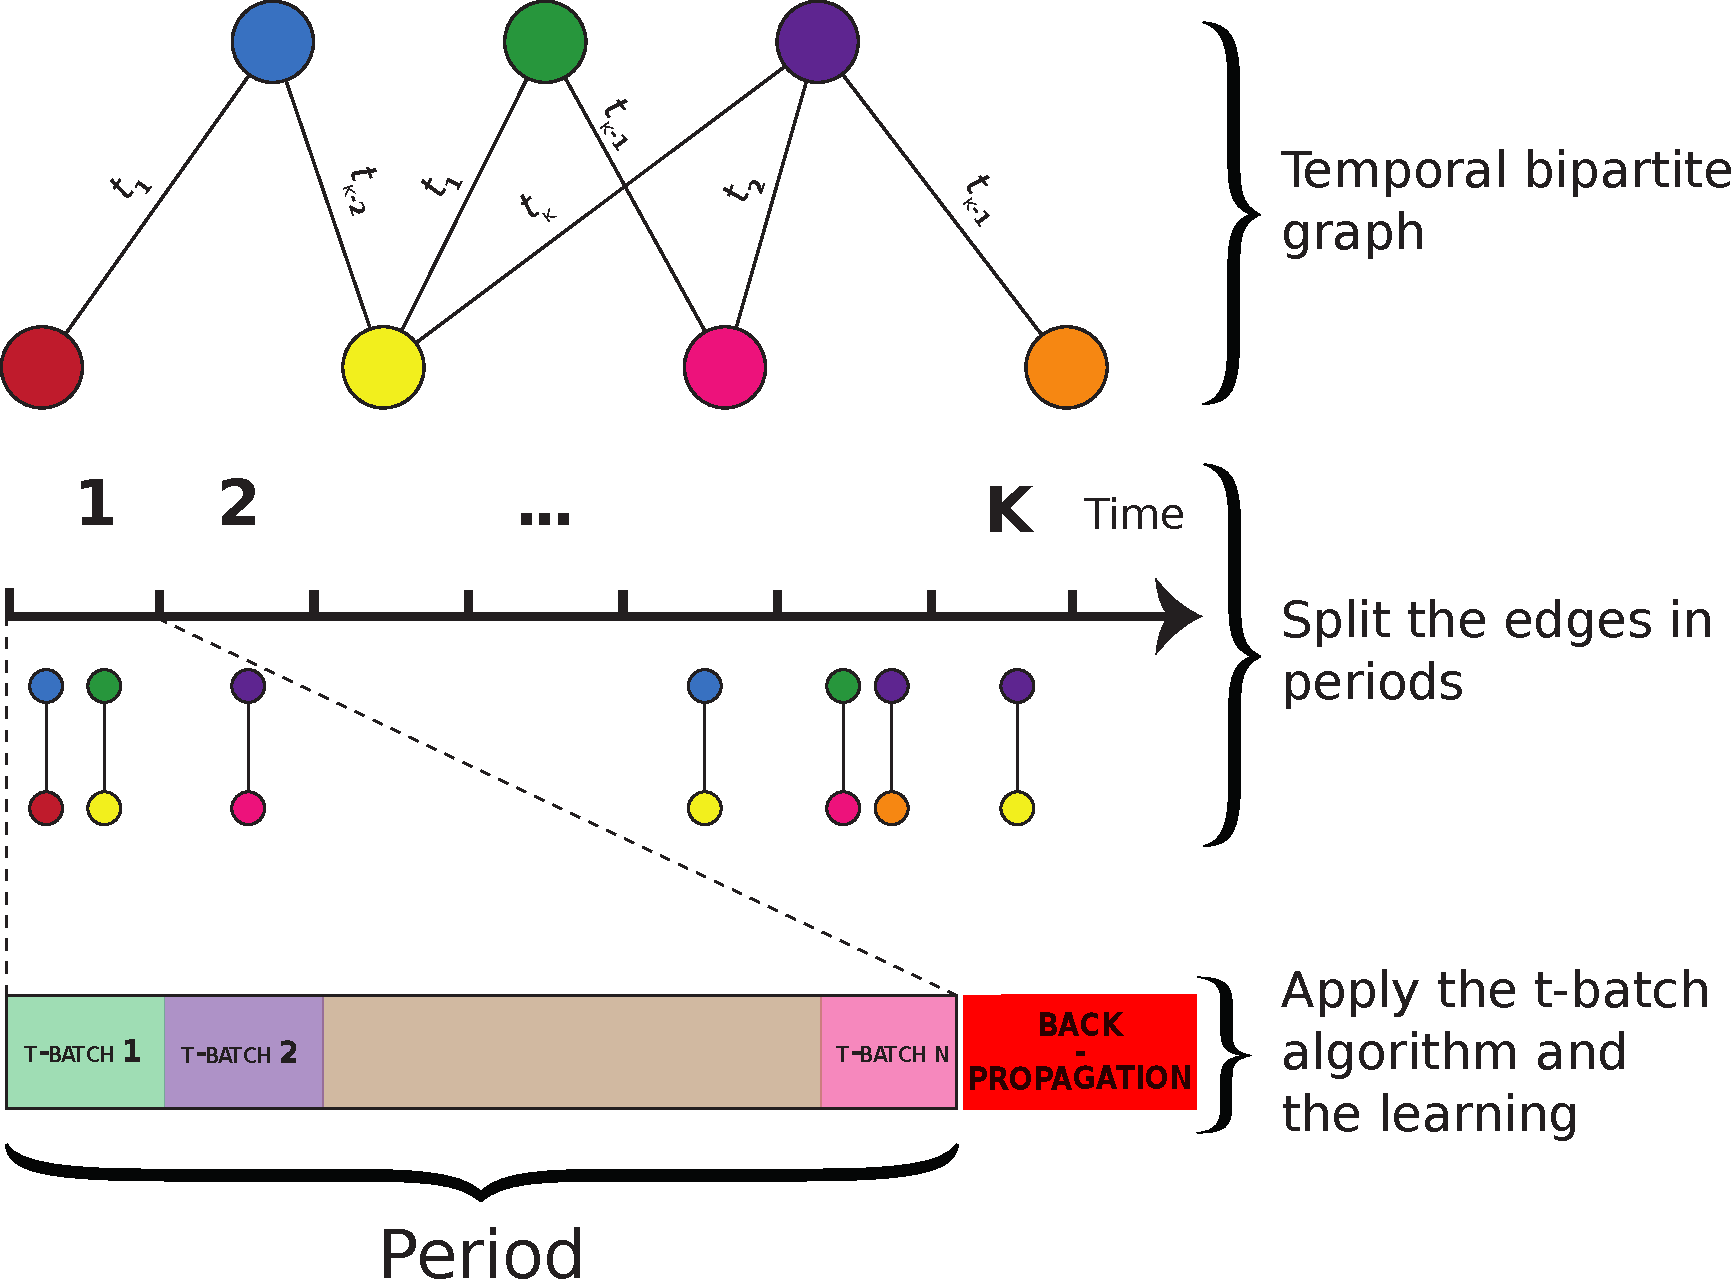
\includegraphics[width=.7\textwidth]{image/pipeline_t-batch.pdf}
    \caption{Pipeline of the \texttt{t-batch} algorithm}
    \label{pipeline_t-batch}
\end{figure}

\subsubsection{Evaluate JODIE model}

The prediction and evaluation stage are just as special as the learning stage. In the evaluation, there is still a "learning" because during the predictions, the model will update itself respecting the time of the periods defined by \texttt{split}. This evaluation is done thanks to the function \textbf{evaluate} of the file \textbf{evaluate.py}. During the evaluation, we do not apply the \texttt{t-batch} algorithm on the remaining interactions, but we will treat them one after the other (figure \ref{pipeline_t-batch} not t-batch but interaction just before the back-propagation).

From a temporal bipartite graph, we proceed in the same way as for learning, we separate the edges in temporal order. Then, we will separate the data into periods and we will process the interactions one after the other. The periods are defined with the hyper-parameter \texttt{split} as for the periods of the \texttt{t-batch}. In addition to all the learning steps in the evaluation, we add a prediction step. According to the prediction task, we will predict a probability of a user's state change using the function \textbf{predict\_state} in the file \textbf{model.py}. Otherwise we will predict an embedding and look for the item which has its closest embedding in terms of Euclidean distance. Finally, we will calculate the metrics to obtain the validation and generalization error.

\subsection*{Datasets}
 % dire que les données sont données par les auteurs mais qu'elles ont un format bizarre et qu'il a fallu traiter les données.
 
The data sets that were used in the original article were also used in this work. The authors of the article give the datasets. \\

\textbf{Reddit~\cite{Reddit} post dataset}: this public dataset consists of one month of posts made by users on subreddits. We selected the 1000 most active subreddits as items and the 10000 most active users. We convert the text of each post into a feature vector representing their Linguistic Inquiry and Work Count~\cite{pennebaker01LIWC} (LIWC) categories.\\
\textbf{Wikipedia~\cite{Wiki} edits}: this public dataset is one month of edits made by edits on Wikipedia pages. We selected the 1000 most edited pages as items and editors who made at least 5 edits as users (a total of 8227 users). Similar to the Reddit dataset, we convert the edit text into a LIWC feature vector.\\
\textbf{LastFM~\cite{10.1007/978-3-642-33486-3_5lastFM} song listens}: this public dataset has one month of who-listens-to-which song information. We selected all 1000 users and the 1000 most listened songs. In the dataset, interactions do not have features.\\
\textbf{Reddit bans}: Reddit post dataset with ground-truth labels of banned users from Reddit. This gives 366 true labels (=0.05\%).\\
\textbf{Wikipedia bans}: Wikipedia edit data with public ground-truth labels of banned users. This results in 217 positive labels (=0.14\%).\\
\textbf{MOOC~\cite{mooc} student drop-out}: this public dataset consists of actions done by students on a MOOC online course. This dataset consists of 7047 users interacting with 98 items. There are 4066 drop-out events (=0.98\%). All datasets and their details are shown in table \ref{description data}. \\

\setlength\tabcolsep{0.12cm} % changer l'écart entre les colonnes pour faire rentrer sur la bonne largeur.
\begin{table}[H]
    \centering
    \ra{1.3}
    \begin{tabular}{@{}lrrrrcc@{}}
    \toprule
    & Users & Items & Interactions & State changes & Action repetition & Features size \\
    \midrule
    Reddit & 10,000 & 984 & 672,447 & 366 & 79\% & 172 \\
    Wikipedia & 8,227 & 1,000 & 157,474 & 217 & 61\% & 172 \\
    LastFM & 980 & 1,000 & 1,293,103 & -\textcolor{white}{0} & 8.6\% & 2 \\
    MOOC & 7,047 & 97 & 411,749 & 4,066 & - & 4 \\
    \bottomrule
    \end{tabular}
    \caption{Description of the datasets that were used in this project}
    \label{description data}
\end{table}
\setlength\tabcolsep{6pt} % default value: 6pt

The authors of the original paper created their own datasets. Thus, a dataset has the following format :
\begin{itemize}
    \item A line represents an interaction or an edge
    \item Each line is described by a user, an item, a timestamp, a state label and features
    \item The timestamp is in cardinal number format
    \item The state label is 1 if the user changes state and 0 otherwise. If there are no state labels, use 0 for all interactions
    \item Features can be as long as desired and of dimension at least 1. If there is no feature, use 0 for all interaction
\end{itemize}
A negative point about the data sets is that the variable names are not in the right places and this creates errors when using them. That is why we created a function called \textbf{fetch\_datasets} in the file \textbf{preprocessing.py} which allows to have correct variable names which have the following format: \texttt{user, item, timestamp, labels, f\_1, ..., f\_$n$} with $n$ the number of features.\\

\subsection*{Hyperparameters}

% ce sont nos hyperparamètres a tester ! Eux n'ont pas fait de recherche pour la taille des embeddings juste ils testent la robustesse du modèle en faisant varier la taille des embeddings sur lastFM

As described in the model descriptions section, the model has several hyperparameters like epoch number, dynamic embedding size, learning rate, \texttt{split}, $\lambda_U$ and $\lambda_I$. Initially the hyperparameters were chosen as in the original article as follow.

\begin{itemize}
    \item Embedding size: $32, \, 64, \, \textbf{128}, \, 256$
    \item Epoch, learning rate, $\lambda_U$ and $\lambda_I$: $50, \, 1e-3, \, 1, \, 1$ respectively
    \item \texttt{Split}: $500$
\end{itemize}

Only the size of the dynamic embeddings have been studied and chosen using a grid search. The other hyperparameters are just given without any justification.

\subsection*{Extended experiments}

% dire les expériences en plus et insister sur le split.

Of all these hyper-parameters, the one that caught our eye the most was \texttt{split}. Indeed, \texttt{split} is used to define the frequency at which t-batches are created and the JODIE model is trained. It is important to choose its value well to have enough data in a period. To test this hyper-parameter, we set the other hyper-parameters to $50$ epoch, $\lambda_U = \lambda_I = 1$, learning rate = $1e-3$ and the size of the embeddings to $128$, and we test these $5$, $500$ and $50000$ for the value of \texttt{split}. We define \texttt{split} as follows:
\texttt{split} is used to split the dataset for a specific period of time. The authors use it as follows : $\frac{\text{time}_{\text{end}} - \text{time}_{\text{start}}}{\text{\texttt{split}}}$

\section*{Results}

In this section, we will present the results obtained with replication. First, we tried to replicate the results for the user's state change prediction on all available datasets. The strategy  was to predict only with the model weights obtained in the last learning epoch while the authors decided to keep the best epochs weights. For this prediction task, other embedding sizes were tested like 8, 16 and 32. Then, we tried to reproduce the results for the future interaction prediction using the same strategy as for the state prediction. Then a second part was devoted to adding results that are not present in the original paper like the importance of the \texttt{split} hyper-parameter.

\subsection*{Core replication results}
The first part of the results concerns the prediction of the user's state change. The model has for hyperparameters a \texttt{split} of $500$, $\lambda_U = \lambda_I = 1$ as those in the original paper and the embedding size varies. We present the results obtained for embeddings of size $32$, $128$ and $256$ as well as the results of the original paper in the table~\ref{result-state}.

\begin{table}[H]
    \centering
    \ra{1.3}
    \begin{tabular}{@{}lcrrrr@{}}
    \toprule
    & JODIE & \phantom{abc} & \multicolumn{3}{c}{Replications} \\
    \cmidrule{2-2} \cmidrule{4-6}
    & 128 && \multicolumn{1}{c}{32} & \multicolumn{1}{c}{128} & \multicolumn{1}{c}{256} \\
    \midrule
    Reddit & $\boldsymbol{0.599}$ && $0.563 \pm 0.013$ & $0.586 \pm 0.018$ & $0.577 \pm 0.012$\\
    Wikipedia &$\boldsymbol{0.831}$ && $0.728 \pm 0.010$ & $0.738 \pm 0.030$ & $0.711 \pm 0.008$\\
    MOOC &$\boldsymbol{0.756}$ && $0.688 \pm 0.006$ & $0.718 \pm 0.021$ & $0.711 \pm 0.004$\\
    \bottomrule
    \end{tabular}
    \caption{Results: user state change prediction}
    \label{result-state}
\end{table}

We observe for the Reddit dataset, a performance of $0.586$ AUC for the reproduction against $0.599$ in the original paper. We also notice a  $0.718$ AUC  for the MOOC dataset results which is close to the $0.756$ AUC obtained in the original paper. For Wikipedia dataset, we can observe a performance of $0.738$ AUC for the reproduction and $0.831$ AUC for the original model. On the Reddit, Wikipedia and MOOC datasets, we see a standard deviation of $0.018$, $0.030$ and $0.021$ respectively for an embedding size of 128. We can explain this difference by the fact that the authors of JODIE evaluated their models on each epoch and chose the best performance in validation while our results come from the 50 and last epoch. This can explain the difference between their results and our results but this difference remains nevertheless marginal.
We can see that if we increase the size of the embeddings to 256, the results degrade slightly. This can be due to size of the embeddings which is too big which allows fitting some noise from the data. Conversely, if the size of the embeddings is 32, the results are worse. This can be explained by the fact that the embeddings are too small and lack information to make a good prediction.\\

For the prediction of future interaction, we used the same hyperparameters as for the state prediction. We present the obtained results and the results of the original paper in the table~\ref{result-interaction}

\begin{table}[H]
    \centering
    \ra{1.3}
    \begin{tabular}{@{}lccccc@{}}
    \toprule
    Dataset\hspace*{3em} & JODIE & \phantom{abc} & \multicolumn{3}{c}{Replications} \\
    \cmidrule{2-2} \cmidrule{4-6}
    & 128 && \multicolumn{1}{c}{32} & \multicolumn{1}{c}{128} & \multicolumn{1}{c}{256} \\
    \midrule
    \multicolumn{1}{l}{\hspace{-0.2cm}\textbf{Reddit}} \\
    {\quad \small MRR} & $\boldsymbol{0.726}$  && $0.711 \pm 0.007$ & $0.719 \pm 0.008$ & $0.684 \pm 0.005$ \\
    {\quad\small Recall@10}  &$\boldsymbol{0.852}$ && $0.810 \pm 0.020$ & $0.830 \pm 0.020$ & $0.747 \pm 0.011$\\
    \multicolumn{1}{l}{\hspace{-0.2cm}\textbf{Wikipedia}}\\
    {\quad\small MRR} &$0.746$ && $\boldsymbol{0.763} \pm 0.005$ & $\boldsymbol{0.764} \pm 0.002$ & $\boldsymbol{0.763} \pm 0.004$  \\
    {\quad\small Recall@10}  & $0.822$ && $\boldsymbol{0.829} \pm 0.005$ & $\boldsymbol{0.833} \pm 0.004$ & $\boldsymbol{0.827} \pm 0.004$\\
    \multicolumn{1}{l}{\hspace{-0.2cm}\textbf{LastFM}} \\
    {\quad\small MRR} &$0.195$ && $\boldsymbol{0.311} \pm 0.001$ & $\boldsymbol{0.313} \pm 0.002$ & $\boldsymbol{0.312} \pm 0.001$ \\
    {\quad\small Recall@10}  & $0.307$ && $\boldsymbol{0.455} \pm 0.003$ & $\boldsymbol{0.483} \pm 0.047$ & $\boldsymbol{0.453} \pm 0.002$\\
    \bottomrule
    \end{tabular}
    \caption{Results: future interaction prediction}
    \label{result-interaction}
\end{table}

We notice that only the results on the Reddit dataset are slightly lower than in the original paper. On these data, we obtained 0.719 in MRR and 0.830 in Recall@10. However, these results remain close to those obtained by the authors with 0.726 in MRR and 0.852 in Recall@10. For the Wikipedia and LastFM datasets, we can see that our results outperformed the authors' results with 0.764 in MRR and 0.833 in Recall@10 and 0.313 in MRR and 0.483 in Recall@10 respectively. These differences can be explained by the choice to evaluate the last epoch and not to choose the best performance on the validation, nonetheless these differences remain small. 

To go further in the replication and reproduction, we will also reproduce two figures that show that the robustness of JODIE model (see fig~\ref{percentage-train}. The first figure will concern the prediction of future interaction on the Wikipedia dataset by plotting the MRR. For this figure, we varied the percentage of the training set from 10\% to 80\% with 10\% step. The second figure will be on the same dataset but for the prediction of user state change. For this, we varied the percentage of the training set from 20\% to 60\% in 10\% steps.

\begin{figure}[H]
    \centering
    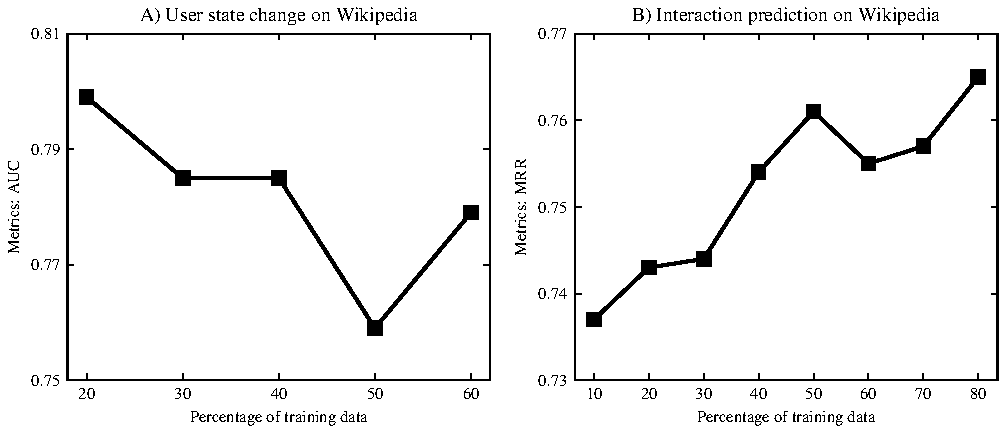
\includegraphics[width = \textwidth]{image/percentage_train.pdf}
    \caption{Robustness of JODIE replication: the figure on the right compare the MRR of JODIE replication with baselines on interaction prediction task, by varying the training data size. The figure on the left shows the AUC of user state change prediction task by varying the training data size.}
    \label{percentage-train}
\end{figure}

\textcolor{red}{Je ne comprend pas tres bien se que tu veux dire}
We can see on the first figure that shows an increasing curve. The larger the training set is, the better is the model in the prediction of future interaction. If we were to compare the curve obtained by the authors of the paper and ours, we could say that the general shape is similar. For the second [figure which one], the curve is decreasing. The larger the training set is, the more the model is wrong. In state prediction, there is very few change of state so the model will tend to predict more the majority class when the training set is smaller and does not contains enough changing state cases. This is even more pronounced when the training set get even smaller.\\

Additionally, we test the robustness of the model for variations in the size of the embeddings (see fig~\ref{emb-size}). The figure on the left shows the MRR results of predicting future interactions for the datasets LastFM and Wikipedia and the figure on the right shows the same results but in recall@10.
\begin{figure}[H]
    \centering
    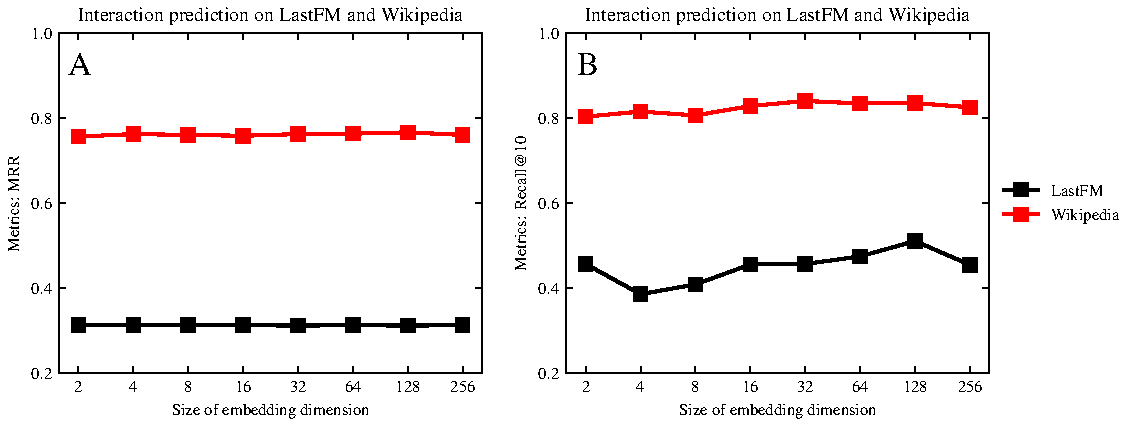
\includegraphics[width = \textwidth]{image/lastFM-wiki.pdf}
    \caption{Robustness of JODIE replication}
    \label{emb-size}
\end{figure}
In the original paper, the authors performed this experiment for embedding sizes of 32, 64, 128 and 256 on LastFM. Here , we proposed to do the same experiment but with two additional embedding sizes 8 and 16 but also to add a dataset which is Wikipedia, to test if the claiming of the original paper is generalizable. We see that whatever the size of the embeddings, we obtain stable MRR performances for both datasets. To go further, we decide to draw the same curves but for the recall@10. On this figure, we can see that there is indeed an increase in performance. As we can see the robustness of the model is depending on the metric choice.

We can say that their model outperforms the existing models on these 4 datasets and replication and reproduction are validated.

\subsection*{Additional result not present in the original paper}

To go further, we decided to test the impact of the \texttt{split} hyper-parameter. As a reminder, the original study does not consider \texttt{split} as a hyper-parameter but as a fixed value of 500. The following figures show the importance of choosing this hyper-parameter. To do so, we predict the user state change on MOOC dataset with several embedding sizes 8, 16 and 32 and different \texttt{split} 5, 500 and 50000. We can see in figure~\ref{split}, for any embedding size, that the performance is increasing when the \texttt{split} values is high. By increasing this \texttt{split} value from 5 to 500, we have increased the performance by 0.14 in AUC for the different sizes of embedding. Going from 500 to 50000, increased the performance by 0.08. We can say that the choice of this hyper-parameter is important to have better performance. We can explain this improvement by the fact that the model will do back-propagation after each time step defined by \texttt{split}. So if we increase the \texttt{split} number, we increase the number of back-propagation. This suggest that higher values of this parameter allows to enhance the performance but the choice of it must been done considering the running time and the complexity which are increasing significantly when the \texttt{split} get larger.

\begin{figure}[H]
    \centering
    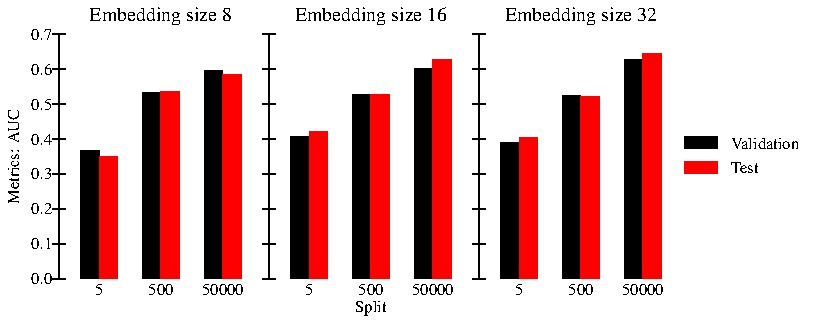
\includegraphics[width = \textwidth]{image/split.pdf}
    \caption{Comparison the robustness of the JODIE model as a function of the hyper-parameter \texttt{split}.}
    \label{split}
\end{figure}

\section*{Conclusion}
With our work we are able to successfully reproduce the results obtained by the authors of the original paper. As explained in the previous section, some of our results differ slightly from those in the paper. This can be explained by a variation due to the initialization but also by the evaluation of the last epoch for the replication while the authors of the paper evaluated each epoch and chose the best performance on the validation. We can say that the JODIE model outperforms the state of the art methods.\\
Our replication allowed to make a more readable code, easily reusable and easily adjustable for all the hyper-parameters combinations.\\
We also tested the importance of the hyper-parameter \texttt{split}. It was concluded that it is important to choose well to obtain better results. The highest performance was obtained with the largest value but a learning time that is longer. This hyper-parameter must be adjusted taking into account a complexity-performance trade-off.\\
In terms of perspectives, it would be interesting to use the focal loss~\cite{https://doi.org/10.48550/arxiv.1708.02002}. We use this loss in cases of unbalanced class. This loss allowed to have better results in these cases.